% тут сейчас будут очевидные коментарии
\documentclass[12pt,a4paper]{article}
\usepackage[utf8]{inputenc}				% кодировка утф8
\usepackage[T2A]{fontenc}
\usepackage[russian]{babel}				% локализация
\usepackage{misccorr}					% пакет с дополнительными настройками для соответствия правилам отечественной полиграфии (не знаю, нужен ли, тупо скопипастил)
\usepackage{color}
\usepackage{graphicx}			% чтоб картинки вставлять
\usepackage{amsmath}					% для формул
\usepackage{amsfonts}
\usepackage{amssymb}
\usepackage{listings}                   % для вставок кода
\usepackage{hyperref}                   % оформление ссылок
\usepackage{blindtext}
%\usepackage[obeyspaces]{url}        % для путей и ссылок


\graphicspath{ {pic} }       % путь до картинок

%\color[named]{BrickRed}
%\pagecolor[named]{Green}

\begin{document}

\begin{titlepage}
\title{Разработка USB устройства ввода в Linux}
%\thanks{Version 1.0}
\author{Михаил Белкин}
\maketitle
\end{titlepage}

\tableofcontents
\newpage

\section{Введение}
    USB достаточно свежая технология (USB 1.1 - 1998г., USB 2.0 - 2000).
    Задумывалась как универсальная шина для компьютерной периферии.
    И в реальности так оно и оказалось, почти все устройства, даже те что
    раньше были только встроенными теперь можно купить и в USB варианте,
    например, сетевую карту. Да и вообще на сегодняшний день сложнее найти
    клавиатуру без USB разъема, чем с ним, хотя для клавиатур и мышек когда
    то задумывался отдельный стандартный разъем.
    Я же остановлюсь на чем попроще и соберу геймпад.\\
    А данная статья, в отличии от остальных рассматривает процесс разработки
    всесторонне. Также нужно сказать что я не ставил цели написания \\
    подробной документации на все те программы, которые я использовал. Их вы
    можете найти по ссылкам в списке литературы, в данной статье только
    комментарии к коду.

\section{Схемотехника.}
\subsection{Выбор редактора схем.}
    Разработка схемы производится в KiCAD, это очень легковесный и компактный
    opensource редактор. Но при этом, несмотря на его внешнюю простоту, редактор
    как будто бы кричит нам "Я ничем не хуже чем этот ваш Altium и уж тем более
    Eagle". Поддерживается редактирование многослойных плат, так же используется
    профессиональный подход, при котором схема устройства и печатная плата
    редактируются отдельно. Так же он очень нетребователен к ресурсам
    компьютера.\\
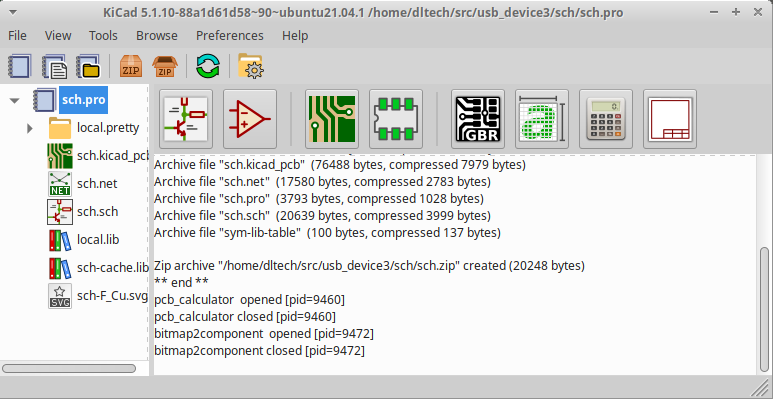
\includegraphics[width=10cm]{kicad1.png}\\
    К редактору имеется собственная библиотека компонентов, которая включает в
    себя компоненты всех популярных производителей. Но если вы принесли
    с китайского базара какую то экзотику, компонент придется разработать
    самостоятельно.\\
    Вывод шаблона печатной платы возможен во всех удобный форматах, включая pdf.
    Так же и Gerber и векторный svg, последнее очень удобно для печати шаблона
    на принтере. Единственное неудобство это не возможность сразу выводить схему
    в растровом формате, приходится самостоятельно конвертировать из svg.

\subsection{Установка редактора и библиотек.}
    Установка редактора в Ubuntu Linux производится очень просто, имеется
    отдельный ppa репозиторий с последней стабильной версией. В то время как
    наиболее полный набор библиотек компонентов можно скачать с гитхаба.\\
    Набор команд для установки KiCAD:
\lstset{language=bash}           % Задаем язык исходного кода
\begin{lstlisting}
sudo add-apt-repository --yes ppa:kicad/kicad-5.1-releases
sudo apt update
sudo apt install --install-recommends kicad
\end{lstlisting}
    Надеюсь устанавливать git вы умеете и про команду git clone вы тоже знаете.
    Вот ссылки на репозитории с библиотеками компонентов KiCAD:\\
    \url{https://github.com/KiCad/kicad-library}\\
    \url{https://github.com/KiCad/kicad-footprints}\\
    \url{https://github.com/KiCad/kicad-symbols}\\
    \url{https://github.com/KiCad/kicad-packages3D}\\
    Установив редактор и добавив библиотеки вы сможете открыть проект со схемой
    устройства
    \href{https://github.com/dltech/usb_device3/tree/main/sch}{по аресу}

\subsection{Выбор элементной базы.}
\subsubsection{Микроконтроллер}
    Для наиболее аккуратной реализации нужен современный микроконтроллер (МК) с
    полноценным аппаратным USB. Совершенно понятно, что таким микроконтроллером
    окажетcя STM32F103C8T6. Мощное ядро ARM Cortex-M3 с их фирменным вложенным
    контроллером прерываний (NVIC) позволит с легкостью справиться с любой
    задачей. А с такой простой как USB геймпад уж тем более. На борту имеется
    64 килобайта FLASH и 20 килобайт SRAM. И этого настолько много, что можно
    вовсе не думать об оптимизации. Теперь о стоимости, когда то я покупал такой
    за 60 рублей, сейчас цена приблизилась к 200, что по прежнему сравнимо по
    стоимости с остальными морально устаревшими микроконтроллерами. Так же в
    пользу данного микроконтроллера говорит наличие подробной
    документации. О том, почему именно F103, тут все просто, это самый дешевый
    МК с USB из тех что может предложить компания ST microelectronics.
\subsubsection{Стабилизатор}
    В шине USB, как известно, 5В, а номинальное напряжение питания МК 3.3В.
    Поэтому необходим понижающий стабилизатор напряжения. Я рассматривал три
    марки стабилизаторов. Они приведены в таблице ниже:
\begin{center}
  \begin{tabular}{ | l | l | l | l | l | }
    \hline
    стаб & $U_{in max}$ & корпус & производитель & особенности \\ \hline
    L78L33 & 30 & SOT-89 & ST microelectronics &  \\ \hline
    AMS1117-3.3 & 15 & SOT-223 & AMS semitech & термозащита \\ \hline
    XC6206-33 & 7 & SOT-23 & TOREX & CMOS \\ \hline
     \end{tabular}
\end{center}
    И если первый давно знаком многим радиолюбителям. То последние два это
    стабилизаторы от китайских производителей, которые появились недавно.
    В целом гораздо больше доверия к старому 78l, как минимум из за его
    большого входного напряжения. К тому же AMS1117 мне
    попадались нерабочими, и очень легко пробивались от скачков напряжения,
    не спасая нагрузку. Но хотелось бы компактней и подешевле, к тому же
    компьютер сам по себе стабильный источник питания. Поэтому я выбрал XC6206.
    Довольно необычный новодел на полевых транзисторах, в то время как другие
    два на биполярных. Ниже приведена его структурная схема, на которой видны
    еще и защитные антистатические стабилитроны.\\
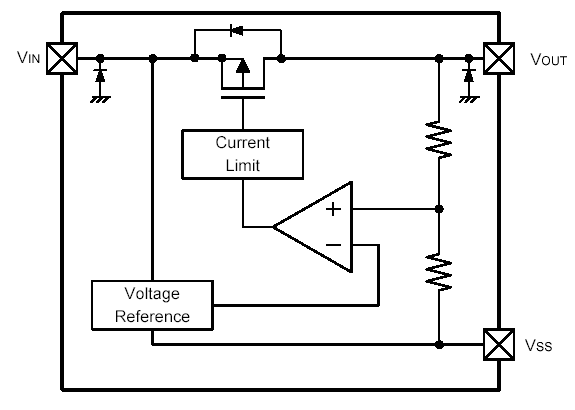
\includegraphics[width=10cm]{6206.png}
\subsubsection{Мелочь}
    На форумах можно услышать совет не ставить кварц в целях экономии. Но в
    в случае с асинхронной шиной кварц нужен для
    стабильной работы устройства. Микроконтроллер можно настроить на работу от
    самого распространенного кварца на 8мГц. Не удивительно, что на алиэкспресс
    сразу же нашелся не только планарный, но и очень компактный вариант.
    Размером как 1206 чип резистор. \\
    Резисторы размером 0402 я успел заказать заранее. А вот шунтирующие
    конденсаторы пришлось выпаивать с донорских плат, потому они не такие
    компактные, как хотелось бы (0805). \\
    Расчетный ток потребления десятки миллиампер, потому для стабилизации
    питания хватит и чип керамики, благо такая есть даже на 10 мкФ.
    На всякий случай установлю токоограничивающий резистор по питанию.
    Основная его цель обезопасить компьютер от случайного короткого замыкания.
    Хотя в дорогих флешках на его месте можно встретить чип предохранитель.
    Продолжу экономить и на разъемах, попросту ограничусь площадками под
    проводки.

\subsection{Особенность схемотехники USB.}
    На сайте можно скачать целый документ, посвященный вопросу распайки USB
    разъема. Основной вопрос заключается в возможности программного отключения
    устройства от ПК. Моё же устройство будет всегда включено, поэтому
    подтяжка линии DP к питанию будет постоянной, и осуществляться резистором,
    а не управляться транзистором и портом микроконтроллера.
    Также важно не забыть про защитные резисторы. Провод у меня используется
    готовый от клавиатуры, потому разъем на плате не нужен.

\subsection{Схема устройства.}
    А вот и схема целиком, как видите, все шины питания подключены и
    заземлены фильтрующими конденсаторами. Кварц с нагрузочными конденсаторами
    в наличии, так же подтянут к земле и порт сброса. Все как советует официальная документация.
    Кнопки джойстика, как видно, подключены к портам напрямую, т.к. внутри МК
    уже имеются резисторы подтяжки к 3.3В. Так же не обошлось и без так
    называемого ''грязного хака``, для упрощения трассировки платы один из
    портов ввода-вывода (28 вывод) использован как вывод земли. Но в этом нет ничего плохого,
    ведь порты после сброса находятся в состоянии с высоким входным
    сопротивлением.\\
    Так же на схеме вы можете увидеть и стандартный разъем SWD для прошивки
    и отладки ПО. Ровно как и подключенный на землю вывод BOOT0 означает
    запуск прошивки из основной flash памяти. \\
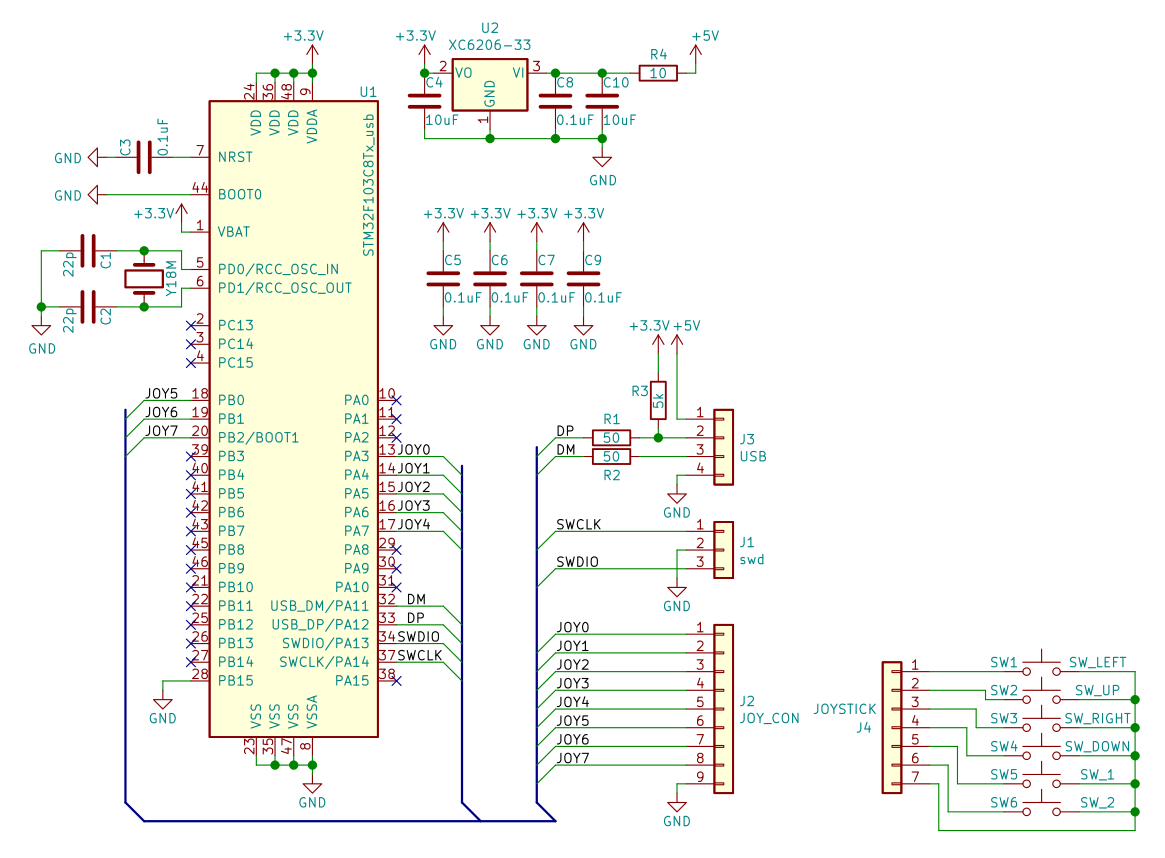
\includegraphics[width=15cm]{sch.png}\\

\newpage
\section{Программное обеспечение.}
    Если по началу, когда эти чипы только появились. Выбора способов написания
    ПО для них было немного. Как правило это были коммерческие среды
    среды программирования под Windows, которые студенты и любители скачивали
    в месте с так называемой таблеткой от жадности. Теперь же выбор
    бесплатных инструментов очень большой. Начиная с официальной среды от
    компании ST, STM32Cube. Которая может не только скачать сама все их
    библиотеки и примеры, но и имеет автоматический конфигуратор периферии (это
    такая штука, которая предлагает настраивать регистры тыкая мышкой).
    И заканчивая сторонними продуктами, таким как AC6 system workbench.
    И эти новые инструменты, в отличии от старых уже кроссплатформенные.
    Так же на гитхабе полно примеров сборки через Makefile.
    А ещё сообщество создало полноценную библиотеку libopencm3 с кучей
    примеров.\\
    Но исходя из того, что пример данного устройства довольно простой. Напишем
    весь код полностью самостоятельно. То есть просто представим, что сейчас
    2007 год и мы только что обнаружили новый чип, на который нету ни сред ни
    примеров.\\
    Можно сказать, что программа для ПК и для микроконтроллера ничем не
    отличается, но на самом деле программы, которые возможно вы писали в школе
    на информатике ориентированы под запуск в операционной системе. От вас
    требуется только код программы, вся остальная рутина уже есть. В случае
    с микроконтроллером все немного по другому.

\subsection{Тулчейн.}
    Когда то просто скачивание и установка gcc была поводом для отдельной статьи.
    Я же отмечу только то, что gcc признает контроллеры на ядре Cortex M3. И
    в ubuntu устанавливается вот такой вот командой:
\begin{lstlisting}
apt install gcc-arm-none-eabi libnewlib-arm-none-eabi
apt install gdb-multiarch
apt install build-essential
\end{lstlisting}
    А наши makefile и скрипты прошивки будут их искать потом как
    arm-none-eabi-gcc, arm-none-eabi-objcopy и gdb-multiarch.
    В остальном даже флаги компиляции в случае с данными микроконтроллерами
    ничем особенно не отличаются.

\subsection{Что нового в CMSIS5.}
    CMSIS это слой абстракции, независимый от производителя. Это не просто
    библиотека, а стандарт взаимодействия с ядром ARM. В библиотеке определены
    главные интерфейсы для инструментов, а также она обеспечивает
    согласованную поддержку устройств. \\
    CMSIS обеспечивает интерфейсы для процессоров и периферии, операционных
    систем реального времени, и компонентов промежуточного программного
    обеспечения. CMSIS включает в себя механизм доставки для устройств, плат,
    и программ, и позволяет комбинировать программные компоненты от разных
    поставщиков. \\
    Важно заметить, что с появлением последней пятой версии она отличается от
    предыдущих, была дополнена и исправлена. Структура проекта CMSIS 5:
\begin{itemize}
    \item Core(M) - стандартизированный API для процессоров Cortex-M
    и периферии. Включает в себя внутренние функции для Cortex-M4/M7/M33/M35P
    SIMD инструкций.
    \item Core(A) - стандартизированный API и базовая система выполнения для
    Cortex-A5/A7/A9 процессоров и периферии
    \item Driver - основные интерфейсы периферийных драйверов для промежуточного
    слоя. Соединяет периферию микроконтроллера со средним слоем что реализует,
    например, стеки связи, файловые системы или графические интерфейсы
    пользователя.
    \item DSP - коллекция библиотек с более чем 60 функций для различных типов
    данных: целочисленных (дробные форматы q7, q15 и q31) и для чисел с
    плавающей точкой одинарной точности (32 бита). Реализации оптимизированы
    для SIMD наборов инструкций для Cortex-M4/M7/M33/M35P
    \item NN - коллекция ядер эффективной нейронной сети разработанные для
    максимизации производительности и минимизации потребления памяти в
    процессорах Cortex-M
    \item RTOSv1 - основной API для операционных систем реального времени
    вместе с примером реализации основанной на RTX. Это включает компоненты
    программ, которые могут работать в нескольких системах RTOS.
    \item RTOSv2 - расширяет CMSIS-RTOSv1 поддержкой Armv8-M, динамическим
    созданием объектов, поддержку мультиядерных систем, бинарного совместимого
    интерфейса.
    \item SVD - периферийное объявление устройства, которое может быть
    использовано для создания периферийной осведомленности в отладчиках
    заголовочных файлах CMSIS-Core.
    \item DAP - прошивка для блока отладчика которая обеспечивает интерфейс к
    порту системы отладки CoreSight DebugAccess
    \item Zone - определяет методы для описания ресурсов системы и для
    разбиения на разделы этих ресурсов в нескольких проектах и областей
    выполнения.
\end{itemize}
\subsubsection{Скачивание CMSIS5}
    Как ни странно, доступны на гитхабе, как обычно, не будем рисковать
    собой, а получим стабильную версию.
\begin{lstlisting}
cd project_dir
git clone https://github.com/ARM-software/CMSIS_5
\end{lstlisting}


\subsection{Компоновщик.}
    Компоновщик это что входит в состав тулчейна gcc, и занимается эта
    утилита сборкой исполняемого модуля из объектных модулей, полученных в
    результате компиляции.\\
    Устройство довольно простое, почему бы по новой не написать целиком все.
    Итак, не совсем целиком. Если игнорирование официальной библиотеки от
    производителя это уже немного глупо, то игнорировать библиотеки создателей
    процессора просто нельзя. Итак, выбран процессор с ядром ARM Cortex M3,
    значит и будем опираться на файл
    \path{CMSIS/Device/ARM/ARMCM3/Source/GCC/gcc_arm.ld}.\\
    Итак, скрипт компоновщика состоит из:
\begin{enumerate}
    \item разметка памяти
    \item определение входной точки
    \item определения секций
\end{enumerate}
\subsubsection{разметка памяти}
    Компоновщик по умолчанию разрешает разметить всю доступную память, включая
    FLASH и SRAM. Для того, чтобы определить область памяти, которая будет
    использована компоновщиком, и избежать использования каких либо других
    областей памяти, существует команда MEMORY. Она
    обозначает расположение и размер блоков памяти. В шаблоне она уже написана,
    от нас требуется занести адреса в переменные.
    Итак, микроконтроллер STM32F103C8T6 имеет 64кБ FLASH, которые начинаются
    с адреса 0x08000000. Значит __ROM_BASE = 0x08000000, __ROM_SIZE = 0x00010000.
    Оперативная память начинается с адреса __RAM_BASE = 0x20000000, размер 20кБ
    __RAM_SIZE = 0x00005000. Размеры стека и кучи оставим без изменений,
    доверимся примеру.
\subsubsection{точка входа}
    Команда ENTRY используется для определения первой исполняемой инструкции.
    Синткасис команды: ENTRY(symbol), где symbol это переменная, которая обычно
    позже переопределяется в коде. В нашем файле программа стартует с адреса
    сброса - Reset_Handler.
\subsubsection{определения секций}
    В скриптах компоновщика переменная точка (.) хранит текущий адрес в памяти,
    в то время как память разделена на секции.
    Команда SECTIONS контролирует то как размечаются input секции в output,
    а также порядок output секций в памяти. Итак, команда SECTION как правило
    используется для определения секции (section definition), которая определяет
    свойства output секций, такие как: ее расположения в памяти, выравнивание,
    содержание, шаблон заполнения, и целевую область памяти. Синтаксис команды
    следующий:
\begin{lstlisting}
SECTIONS {
...
secname start BLOCK(align) (NOLOAD) : AT (ldadr)
    { contents } >region :phdr =fill
...
}
\end{lstlisting}
secname имя секции,\\
start определяет начальный адрес, с которого будет загружаться секция\\
BLOCK(align) выравнивание\\
(NOLOAD) обозначает невозможность загрузки секции во время выполнения программы\\
AT (ldadr) определяет адрес загрузки секции как ldadr\\
>region объявляет секцию как определенную область памяти\\
Служебные слова secname и contents требуются для определения секции, остальные
опциональны.\\
Давайте рассмотрим секцию .text для примера.\\
\begin{lstlisting}
.text :
{
  KEEP(*(.vectors))
  *(.text*)

  KEEP(*(.init))
  KEEP(*(.init))

  /* .ctors */
  *crtbegin.o(.ctors)
  *crtbegin?.o(.ctors)
  *(EXCLUDE_FILE(*crtend?.o *crtend.o) .ctors)
  *(SORT(.ctors.*))
  *(.ctors)

  /* .dtors */
  *crtbegin.o(.dtors)
  *crtbegin?.o(.dtors)
  *(EXCLUDE_FILE(*crtend?.o *crtend.o) .dtors)
  *(SORT(.dtors.*))
  *(.dtors)

  *(.rodata*)

  KEEP(*(.eh_frame*))
} > FLASH
\end{lstlisting}
    .text это имя секции, в секции расположен код. KEEP(*(.vectors)) используется
    для того, чтобы секция векторов прерываний не была оптимизирована (удалена),
    похожий метод применен для секций init, fini, eh_frame*. Напомним, что переменная
    '.' хранит текущий адрес. Таким образом скрипт извлекает из переменной vectors
    конечный адрес векторов, используя переменную точки, и располагает секцию
    vectors в текущей области памяти.
    Так же располагаются секции dtors и ctors по адресам,
    полученным из crtbegin.o и crtbegin?.o.\\
    Секция ctors это список конструкторов (инициализационных функций),
    который подключает функции, инициализирующие данные в момент запуска программы
    (до запуска функции main).
    dtors устанавливает список деструкторов, которые могут быть вызваны при
    завершении программы.\\
    > FLASH обозначает то, что секция text расположена в области FLASH памяти.\\
    Пролистав и эту унылую теоретическую справку, вы можете догадаться,
    что и здесь со стандартным скриптом компоновщика все в порядке,
    ничего трогать не нужно.
\subsection{startup файл}
    Если коротко, то это такой исходник, который не виден обычным пользователям,
    но именно он вызывает функцию main. Вообще возможен и си вариант, но как
    правило пишется на ассемблере. Также есть стандартный в библотеке по пути
    \path{CMSIS_5/Device/ARM/ARMCM3/Source/GCC/startup_ARMCM3.S}.\\
    Все что нам нужно в нем поменять, так это добавить местных векторов
    прерываний. То есть нужно, что бы компилятор знал, с какого адреса запускать
    то или иное прерывание, если оно произойдет.



\subsection{Структура проекта.}

\subsection{Опрос кнопок.}

\subsection{Периферия USB.}

\subsection{Дескрипоры USB.}

\subsection{Стандартный протокол USB.}

\subsection{USB HID}

\subsection{Отладка.}

%\begin{thebibliography}{9}

%\bibitem{lamport94}
%  Leslie Lamport,
%  Addison Wesley, Massachusetts,
%  2nd edition,
%  1994.
%\end{thebibliography}

%\begin{list}
%    \item 78L33
%    \item AMS1117-3.3
%    \item XC6206-33
%\end{list}

\end{document}
